% to compile on Debian/Ubuntu:
% sudo apt install latexmk biber texlive-bibtex-extra texlive-fonts-extra
% latexmk -pdf ik-poster
\documentclass[a4paper,12pt]{article}
\usepackage[utf8]{inputenc}
\usepackage[english]{babel}
\usepackage{amsmath}
\usepackage{graphicx}
\usepackage[top=0.5in, bottom=0.5in, left=0.5in, right=0.5in]{geometry}
%\usepackage[sorting=none,citestyle=numeric-comp,bibstyle=trad-abbrv]{biblatex}
\usepackage{units}
\usepackage{xcolor}
\usepackage[
pdftitle={Local variance optimization for the autonomous regulation of Echo State networks},
pdfauthor={Fabian Schubert, Claudius Gros},
pdflang=en,
pdfborder={0 0 0}
]{hyperref}

\usepackage[comma]{natbib}
\bibliographystyle{apalike}

%\DeclareFieldFormat{titlecase}{#1}


%\addbibresource{abstract.bib}

\begin{document}
\pagestyle{empty}
\begin{center}
  \Large{\textbf{Local variance optimization for the autonomous regulation of echo state networks}}
\end{center}
\vspace{-.08cm}

\section{Summary}
Echo state networks have proven to be a powerful tool in the field of time series prediction~\citep{Jaeger_2001,Lukosevicius_2009}. Several approaches to the optimization of the dynamic reservoir have been investigated in the past, including global tuning for criticality~\citep{Livi_2016}, as well as local adaptation towards a given output distribution~\citep{Schrauwen_2008,Boedecker_2009}. The spectral radius $|\Lambda_{\rm max}|$ of the synaptic weight matrix provides a measure to regulate the network in an appropriate working regime~\citep{Caluwaerts_2013}. We show that $|\Lambda_{\rm max}|$ can be regulated by local homeostasis of the variance $\sigma_y^2$ of neural activity. This variance control operates on the gain of the neural transfer function and its optimization target depends on the variance $\sigma_{\rm ext}^2$ of external inputs: by deriving a relation between recurrent and external input variance, we transferred the explicit spectral radius condition into an implicit expression that defines a manifold in the space of external and recurrent input variances. While our analytically derived condition is only exact for statistically independent external driving across nodes, we have conducted further numerical experiments, suggesting that it also holds under less restrictive conditions. This optimization rule is biologically plausible since it only relies on locally available information. In contrast to previously proposed optimization rules via local intrinsic plasticity, our model relies on the assumption that external and recurrent input signals can be treated as two separate streams of information. The network can hence react autonomously to changes of the input statistics. We demonstrate the importance of this separation by means of network performance ---quantified by a nonlinear memory recall task--- under varying input statistics.
\vspace*{-5pt}
\section{Additional Information}
Our analytical analysis is based on a mean-field approach, where one assumes that all presynaptic neurons are statistical independent.
Optimizing the variance of the neural
activity then consists of solving
%
\begin{equation}
\sigma_{\rm t}^2=\int_{-\infty}^{\infty}
{\rm dx}\tanh^2(ax) N_{\mu,\sigma}(x),
\qquad\quad
\sigma^2=\sigma_{\rm w}^2\sigma_{\rm t}^2+\sigma_{\rm ext}^2\,,
\label{self_consistency_x}
\end{equation}
%
where the distribution $N_{\mu,\sigma}(x)$ of the membrane potential $x$ is a Gaussian, with mean $\mu=0$
and variance $\sigma^2$, which is a combination of external input variance $\sigma_{\rm ext}^2$, recurrent presynaptic variance $\sigma_{\rm t}^2$ and the variance of recurrent synaptic weights $\sigma_{\rm w}^2$. An exact analytic expression for this integral does not exist. An approximation with the correct scaling to second order as well as the right convergence is
\begin{equation}
\tanh^2(x) \approx 1 - \exp\left(-x^2 \right) \; .
\end{equation}
Using this approximation in \eqref{self_consistency_x} and solving the integral yields
\begin{equation}
\sigma^2_{\rm t} = 1 - 1/\sqrt{1+2a^2\sigma^2_{\rm w}\left( \sigma^2_{\rm t} + {\sigma}^2_{\rm ext}/\sigma^2_{\rm w} \right)} \; . \label{eq:gaussian_approx}
\end{equation}
A unit spectral radius translates to the condition $a=\sigma_{\rm w}^{-1}$, allowing us to state a further simplified relation, which is what is required for tuning the network activity into an optimal state:
\begin{equation}
\sigma_{\rm t} \approx \left[\sqrt{\frac{3}{2}} \frac{\sigma_{\rm w}}{\sigma_{\rm ext}} +1\right]^{-1/2} \; . \label{eq:gauss_approx_approx}
\end{equation}
A comparison between a numerical evaluation of this manifold and the analytical results is shown in Fig.~\ref{Fig:theory_simulation_2}A.

Furthermore, we investigated how the network performs under different $\sigma_{\rm t}$ and $\sigma_{\rm ext}$ if given a task that cannot be solved without nonlinear transformations on the input. For this purpose, we defined a XOR-recall task with delay $\tau$ by
\vspace*{-9pt}
\begin{align}
f(t) &= \mathrm{XOR}\left[u(t-\tau),u(t-\tau-1)\right], & \mathrm{XOR}\left[x,y\right] \equiv \begin{cases}
0 & x=y\\
1 & \text{else}
\end{cases} \; .
\end{align}
\vspace*{-7pt}
We defined the total XOR memory capacity by
\vspace*{-1pt}
\begin{align}
\mathrm{MC}_{\rm XOR} &\equiv \sum_{k=1}^\infty \mathrm{MC}_{{\rm XOR},k} , &
\mathrm{MC}_{{\rm XOR},k} \equiv \max\limits_{w_{\rm out}} \frac{\mathrm{Cov}^2\left[\mathrm{XOR}\left[u(t-k),u(t-k-1)\right],y_{\rm out}(t)\right]_t}{\mathrm{Var}\left[\mathrm{XOR}\left[u(t),u(t-1)\right]\right]_t \mathrm{Var}\left[y_{\rm out}(t)\right]_t} \; .\label{eq:MC_XOR}
\end{align}
The results are shown in Fig.~\ref{Fig:theory_simulation_2}B. The maximally achievable performance remains relatively constant over a wide range of $\sigma_{\rm ext}$. This local maximum as a function of $\sigma_{\rm ext}$ is well described by the condition of unit spectral radius and could therefore be homeostatically achieved by means of our implicit relation \eqref{eq:gauss_approx_approx}.
\begin{figure}[t!]
	\centering
	\begin{minipage}[t]{0.46\textwidth}
		\centering
		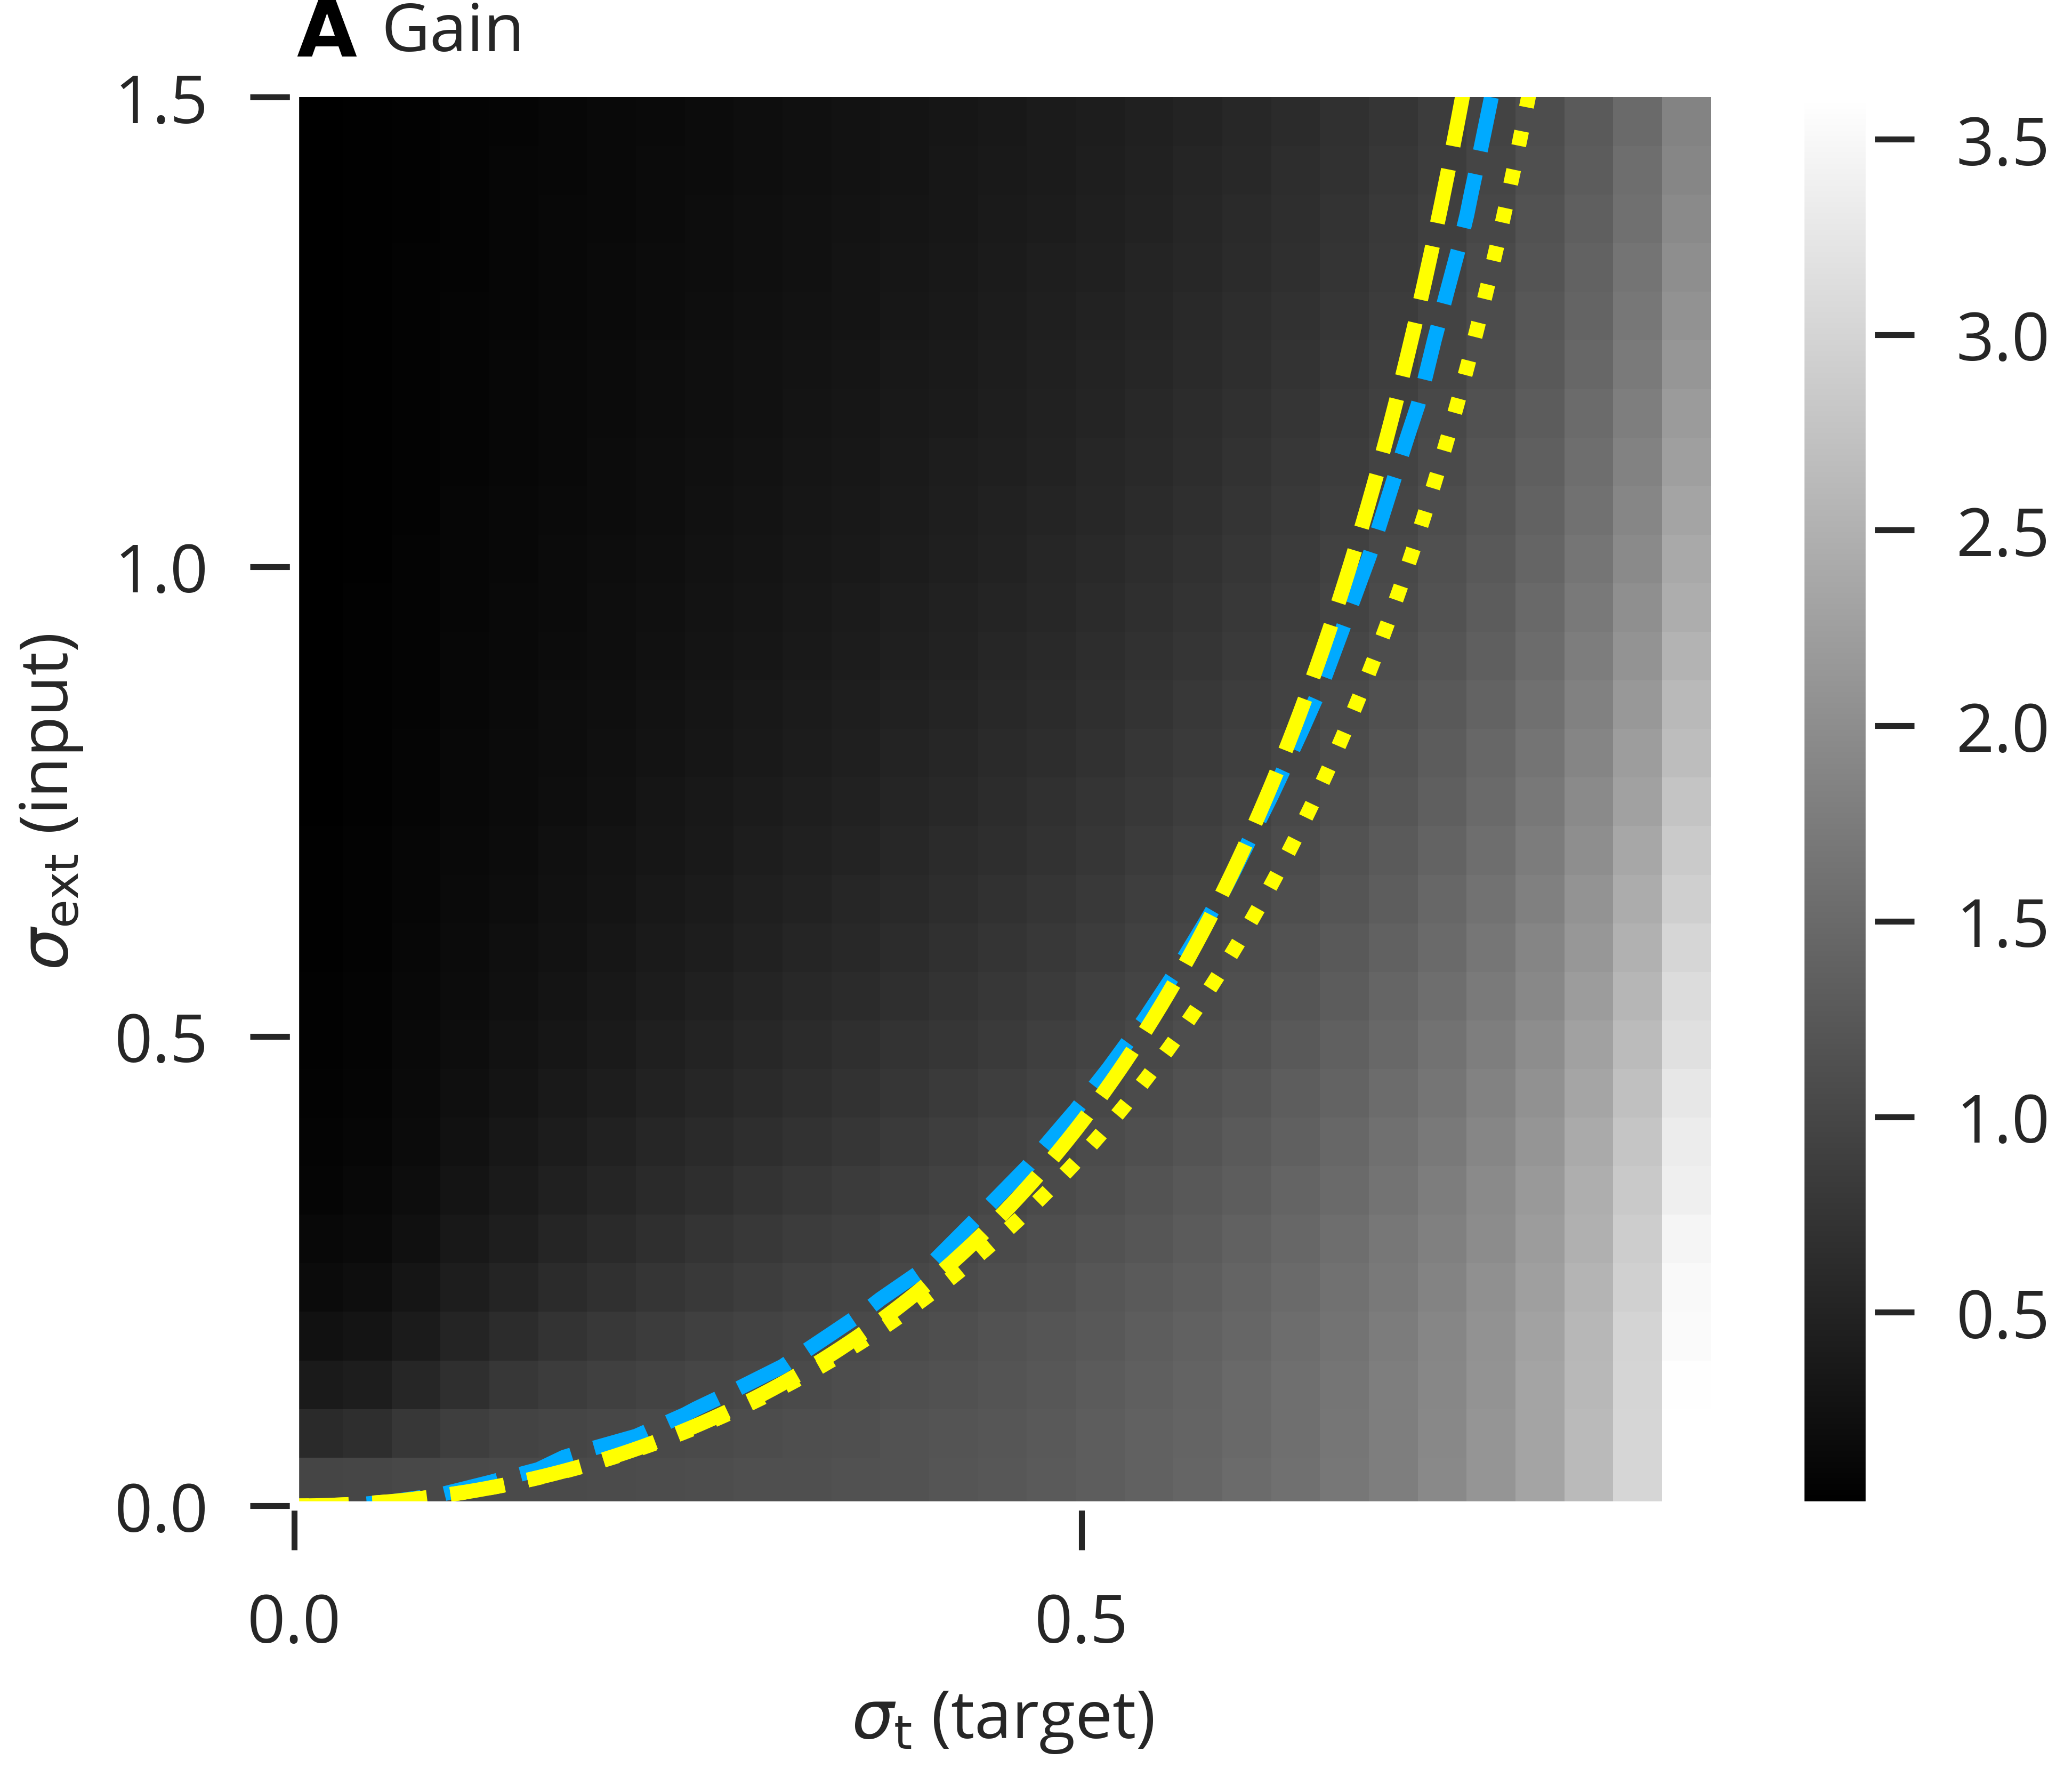
\includegraphics[width=\textwidth]{./plots/theory_simulation_2.png}
	\end{minipage}
	\begin{minipage}[t]{0.42\textwidth}
		\centering
		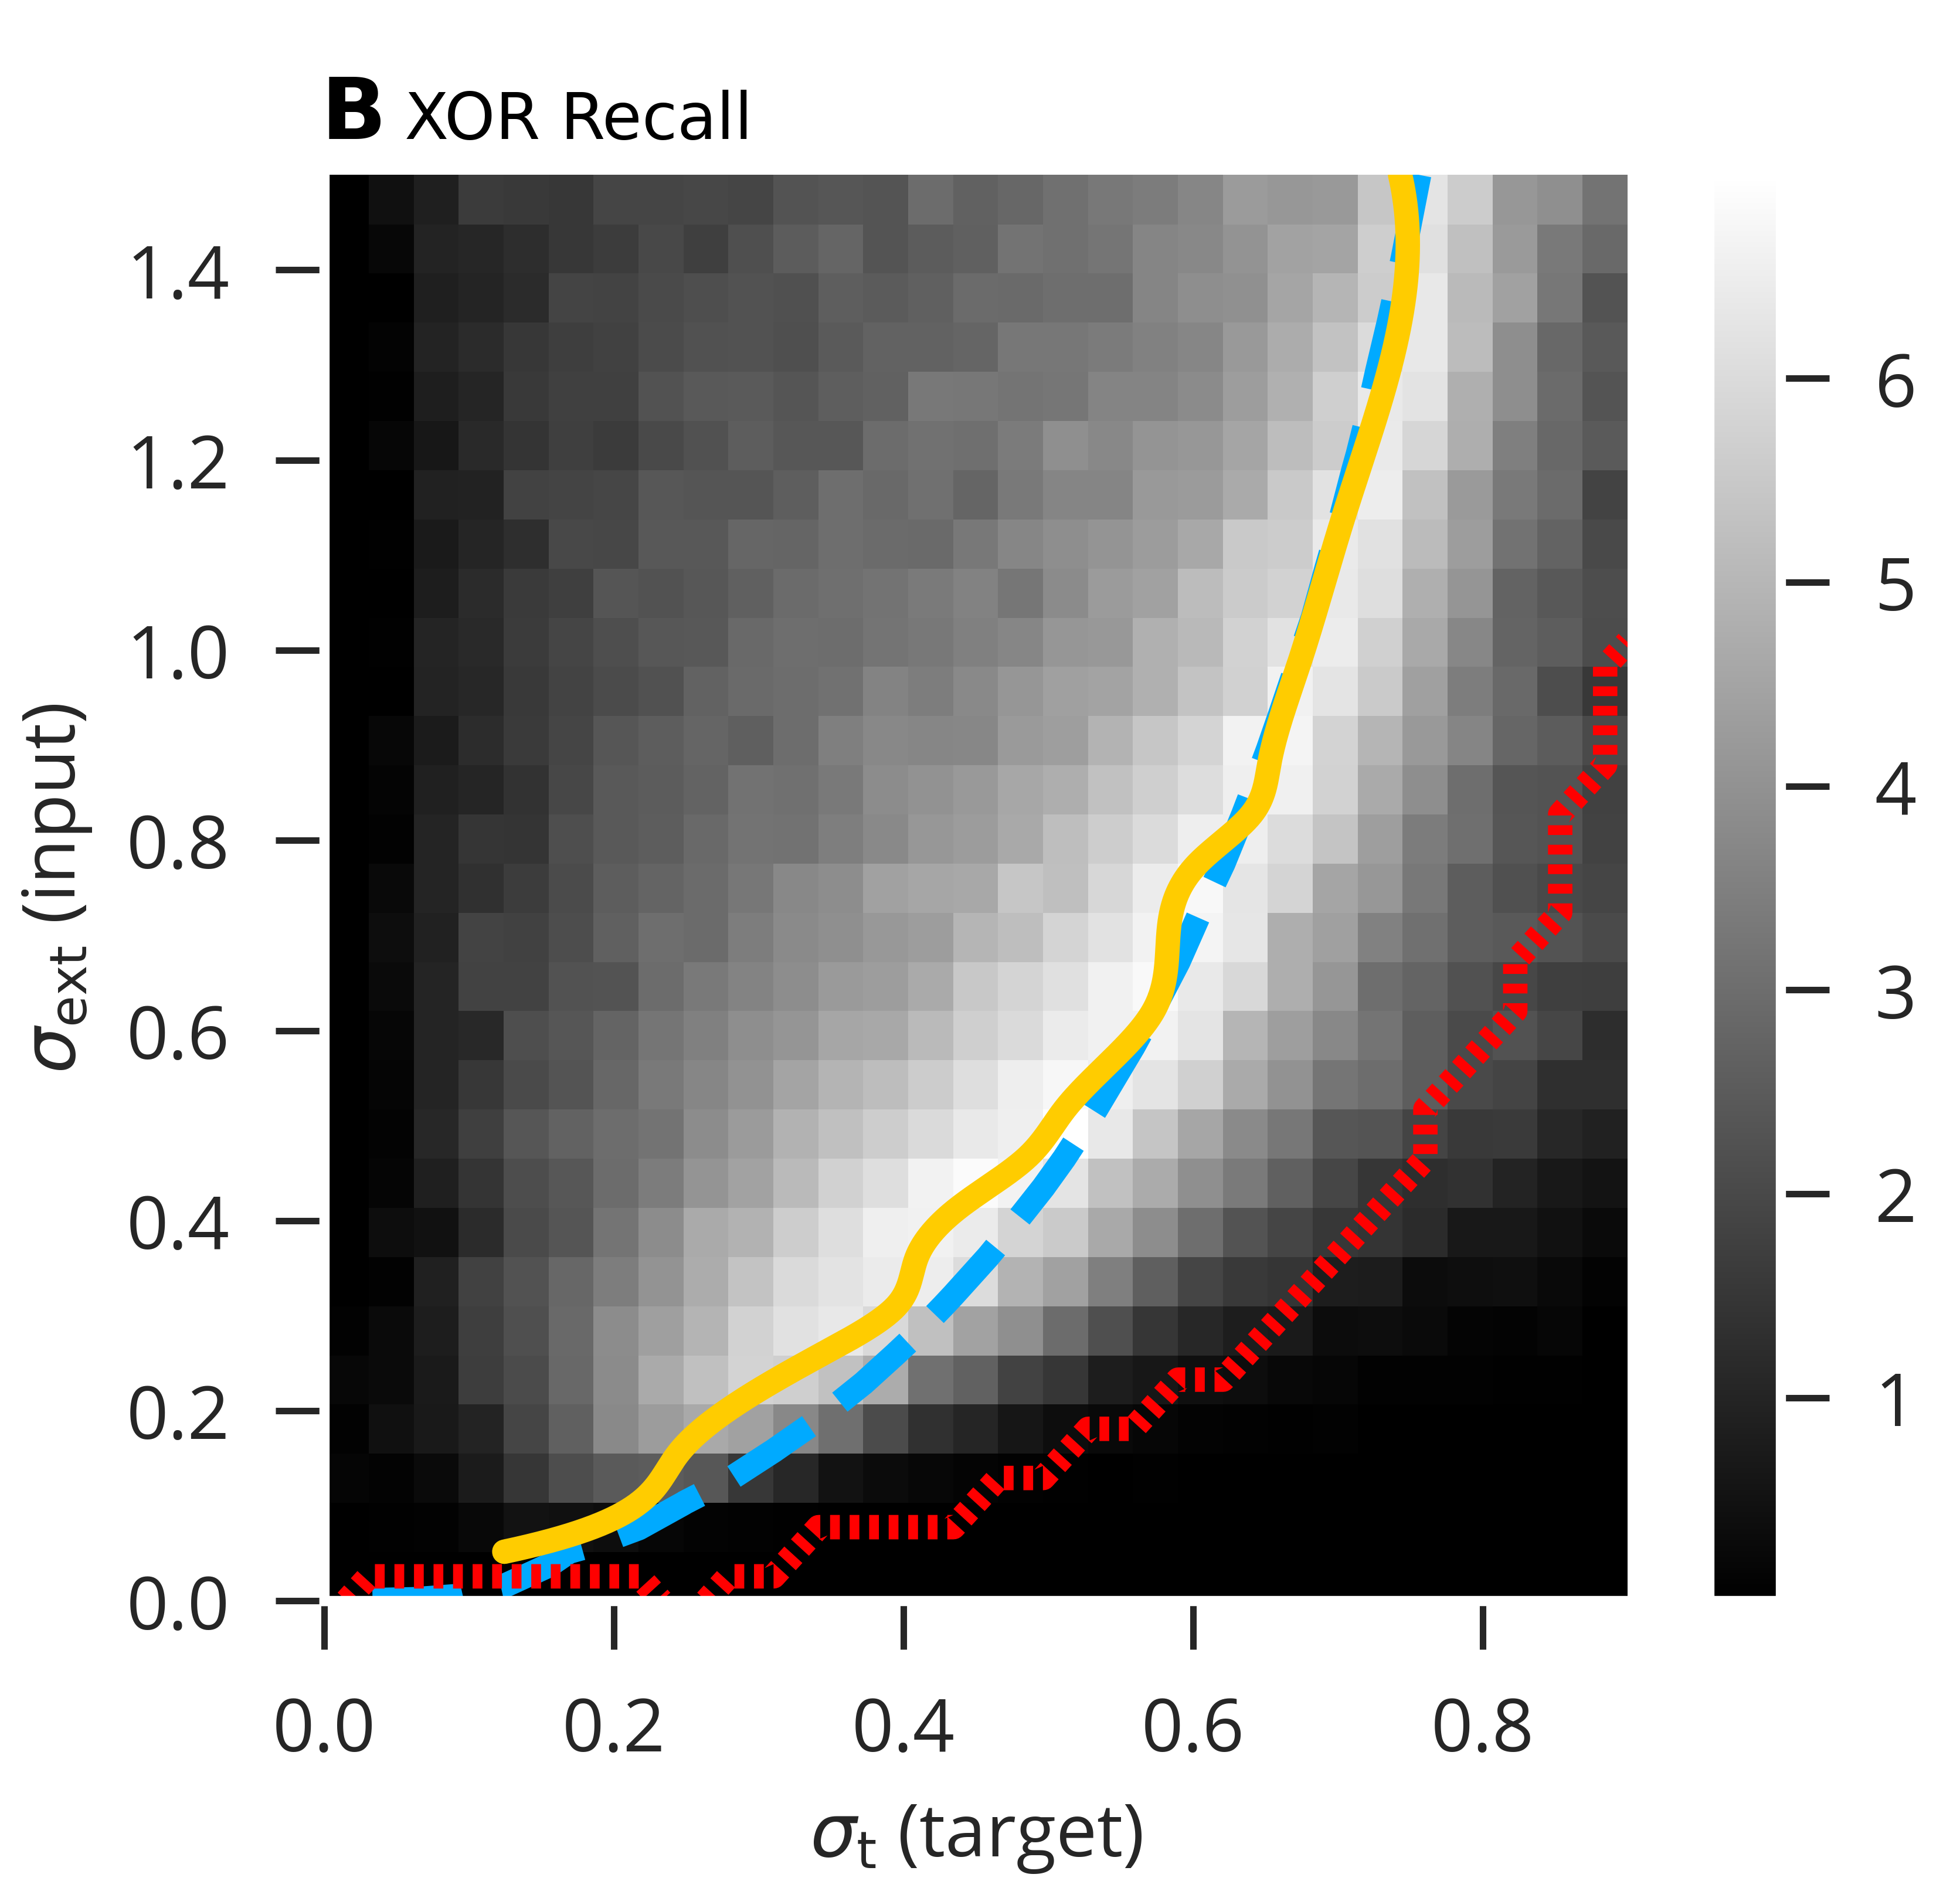
\includegraphics[width=\textwidth]{./plots/xor.png}
	\end{minipage}
	\caption{{\bf Spectral Radius Transition Approximation} {\bf A}: Colormap encodes the spectral radius of recurrent connectivity. Blue dashed line marks unit spectral radius. Yellow dashed line is given by \eqref{eq:gauss_approx_approx}, dotted line by the solution of \eqref{eq:gaussian_approx} for $a=\sigma_{\rm w}^{-1}$. {\bf B}: Colormap encodes $\mathrm{MC}_{\rm XOR}$ as defined in \eqref{eq:MC_XOR}. Blue dashed line as in {\bf A}. The orange line plots the position of maximal $\mathrm{MC}_{\rm XOR}$ for a given $\sigma_{\rm ext}$. Red striped line marks the loss of the Echo-State property.}
	\label{Fig:theory_simulation_2}
\end{figure}



\vspace{-.35cm}
\bibliography{./abstract.bib}

\end{document}

